\subsection{Report of 7 October 2026: literature, feature table, two-output random forest}\label{sec:w1007}

\textbf{Summary.} The question after the first report was whether anyone has predicted NFL scores before, with what data, and how. This week: a literature survey; a catalogue of the data used in the literature against what nflverse provides; the 805-column pre-game feature table with its leakage test (Section~\ref{sec:data}); and a first two-output random forest evaluated walk-forward over sixteen seasons.

\subsubsection{Literature}\label{sec:literature}


The first question raised after the 30 September report was whether anyone has tried to predict NFL scores before, what data they used, and how they thought about the problem. The literature falls into five groups.

\paragraph{Rating models from scores alone.} Harville~\cite{harville1980} fitted a mixed linear model to score differences from 1,320 games and obtained an average error of 10.68 points against 10.49 for the bookmaker. Glickman and Stern~\cite{glickmanstern1998} let each team's strength drift from week to week and season to season in a Bayesian state-space model and matched the Las Vegas line on a 1993 test set. Their handbook chapter~\cite{glickmanstern2017} surveys these methods and recommends entering each covariate as the difference and the average of the two teams' values, which we adopted. FiveThirtyEight's Elo system~\cite{fivethirtyeightelo} is the practical version: one strength number per team updated from margin of victory, with adjustments for home field, rest and the starting quarterback. All of these use only results and the schedule, and all land a few tenths of a point behind the line.

\paragraph{Exact scores and distributions.} Baker and McHale~\cite{bakermchale2013} is the only paper that forecasts both teams' exact NFL scores, with a birth-process model and pre-game covariates; it too performs about as well as the bookmaker. Stern~\cite{stern1991} showed that margin minus spread is approximately normal with standard deviation near 14, which gives the standard conversion from a spread to a win probability; Stern~\cite{stern1994} and Polson and Stern~\cite{polsonstern2015} extend this to the progress of a game and to a market-implied volatility. In soccer, Dixon and Coles~\cite{dixoncoles1997} model scores as correlated Poisson counts and Divos et al.~\cite{divos2018} price in-play bets by risk-neutral methods; the lesson for us is that football scoring is discrete in a way Poisson models do not capture.

\paragraph{Play-level information.} Yurko, Ventura and Horowitz~\cite{yurko2019} defined expected points and win probability from play-by-play data and showed how to attribute them to plays and players. Expected points added per play is the efficiency measure the analytics community has settled on; the nflverse project provides it for every play since 1999 and it is the source of most of our team-form features.

\paragraph{Market efficiency.} Levitt~\cite{levitt2004} showed from a bettor-level dataset that bookmakers do not balance their books but set prices as skilled forecasts that exploit bettor biases, which is why the closing line is hard to beat. Boulier and Stekler~\cite{boulierstekler2003} and Song, Boulier and Stekler~\cite{songboulierstekler2007} compared statistical systems, experts and the betting market and found the market most accurate, with models and experts tied. Zuber, Gandar and Bowers~\cite{zuber1985} and Gray and Gray~\cite{graygray1997} found only small, unstable inefficiencies. Lopez, Matthews and Baumer~\cite{lopez2018} go the other way and use moneylines as the best available measure of team strength. Shin~\cite{shin1993} and Wolfers and Zitzewitz~\cite{wolferszitzewitz2006} show how to read probabilities from odds and from prediction-market prices.

\paragraph{Machine-learning studies.} A systematic review by Galekwa et al.~\cite{mlreview2024} and a number of student projects report accuracies of 70 to 95 percent at picking winners. Where the methods are described, these come from same-game statistics (leakage) or from very small test sets. The closing line picks the winner about 66 percent of the time; nothing credible is far above that. We took two lessons: build an explicit leakage test, and do not expect a flexible learner to add much over a well-specified rating model with 7,000 games.

\paragraph{Data in the literature.} The serious score models use only scores, dates and home field; richer inputs appear in three families: play-level efficiency, quarterback identity and betting lines. Bet-volume data (Levitt; Paul and Weinbach) is proprietary; the Kalshi trade tape is the free equivalent. No paper reviewed uses injuries, snap counts or depth charts in a score model, although Glickman and Stern~\cite{glickmanstern2017} name player-level factors as the obvious gap. Everything the literature uses is available free from nflverse except opening lines and bet splits.

\paragraph{Implication for our design.} Point accuracy for NFL scores is capped near the closing line for every published method. The sensible goal is a calibrated distribution over both scores, consistent across every derived quantity, rather than a lower point error. The suggestions received from Professors Amine and Shasha fit this picture: a multi-output random forest can use every feature without selection, a linear baseline shows whether the forest adds anything, and a probabilistic extension predicting two means, two standard deviations and a correlation is the natural destination for a two-score model.

\subsubsection{Predicting both teams' scores}\label{sec:scoremodel}


\paragraph{Why two scores.}

The object the engine needs is the joint distribution over $(h,a)$. Predicting each team's score is the natural first step: the two predictions locate the centre of that distribution and the spread of the residuals around them gives its width. A model for the margin alone discards the level of scoring; a 30--27 game and a 17--14 game have the same margin and very different distributions of totals and of every strike.

\paragraph{Models and evaluation.}

Table~\ref{tab:models} lists the models. All use the 759 non-market features of Section~\ref{sec:data}; the closing line is a benchmark only. Evaluation is walk-forward: train on every season before $t$, test on season $t$, for $t = 2010,\dots,2025$ (4,363 test games).

\begin{table}[H]
\centering
\small
\begin{tabular}{p{3.6cm}p{6.2cm}p{4cm}}
\toprule
\textbf{Model} & \textbf{Inputs} & \textbf{Role} \\
\midrule
League average & Mean scores in the training seasons & Floor \\
Elo & Results only; implied spread is Elo difference / 25 & Rating baseline \\
Two-output ridge regression & 759 features, median-imputed, standardised, penalty by cross-validation & Linear baseline \\
Two-output random forest & 759 features, 500 trees, at least 20 games per leaf, 30\% of features per split, no tuning & Main model: predicts $(h,a)$ jointly \\
Closing line & Consensus sportsbook spread and total & Benchmark \\
\bottomrule
\end{tabular}
\caption{Models compared. The forest predicts the two scores as a pair: each leaf holds the mean home and away score of similar past games.}
\label{tab:models}
\end{table}

\paragraph{Point accuracy.}

\begin{table}[H]
\centering
\small
\begin{tabular}{lcccc}
\toprule
\textbf{Model} & \textbf{Home score} & \textbf{Away score} & \textbf{Margin} & \textbf{Total} \\
\midrule
League average & 8.09 & 7.91 & 11.18 & 11.02 \\
Elo & -- & -- & 10.38 & -- \\
Two-output ridge & 7.62 & 7.40 & 10.34 & 10.63 \\
Two-output random forest & 7.63 & 7.45 & 10.35 & 10.66 \\
Closing line & -- & -- & \textbf{10.05} & \textbf{10.47} \\
\bottomrule
\end{tabular}
\caption{Mean absolute error in points, walk-forward 2010--2025.}
\label{tab:mae}
\end{table}

The forest explains 10.8\% of the variance of the home score and 9.3\% of the away score out of sample. These numbers are normal for the problem: a single game is mostly noise around a modest signal, and the closing line, with every input a bettor can find, explains only a little more. The forest and the ridge are indistinguishable at every target. On the margin they are 0.03--0.04 points better than Elo and 0.3 points worse than the line (Figure~\ref{fig:mae_season}); the line has the lowest error in 15 of 16 seasons. Straight-up winner accuracy is 64.7\% for the forest, 64.6\% for ridge, 64.5\% for Elo and 66.3\% for the line. Against the spread the forest picks the covering side 49.9\% of the time, as an efficient line implies.

{\color{red}\textbf{Amine comment:} Please report uncertainty for the differences in error on the same games, allowing for dependence over time, and clarify forecast timing relative to the closing line. The table shows gains over Elo of 0.03--0.04 points, not a quarter point.}

{\color{blue}\textbf{Sai comment:} Fixed. The ``quarter of a point'' is corrected to 0.03--0.04 above; the paragraph and Table~\ref{tab:mae_diff} below give paired error differences with i.i.d., week-clustered, season-clustered and Newey--West standard errors (gain over Elo about one standard error; gap to the line seven to eight), and state that model and line are both taken at kickoff.}

Because every forecast is scored on the same 4,363 games, the differences between them are paired, and their uncertainty has to allow for the fact that games in the same week and season are related. Table~\ref{tab:mae_diff} gives the mean difference in absolute margin error for each pair with four standard errors: treating games as independent, clustering by week (271 clusters), clustering by season (16 clusters), and a Newey--West estimate over the game sequence with a lag of four weeks. The four agree closely, which says the game-level errors are nearly uncorrelated once the forecasts are differenced. The gain over Elo, $0.03$--$0.04$ points, is about one standard error and shows up in only 9 or 10 of the 16 seasons: it is not distinguishable from zero. The gap to the closing line, $0.29$--$0.33$ points, is seven to eight standard errors and holds in 15 of 16 seasons. The forest and the ridge differ by $0.01 \pm 0.03$. On timing, every model forecast uses only information available at kickoff and none uses the line (Section~\ref{sec:data}); the closing line is also the kickoff price, so the two are compared at the same instant. The weather columns are the one input strictly observed rather than forecast. Refitting the forest walk-forward without the four weather columns (\texttt{scripts/model\_rf\_noweather.py}) changes the margin error from 10.352 to 10.353 and the total error from 10.663 to 10.676, so nothing in the comparison rests on knowing the weather in advance.

\begin{table}[H]
\centering
\footnotesize
\setlength{\tabcolsep}{4pt}
\begin{tabular}{lrrrrrrc}
\toprule
\textbf{Difference in MAE} & \textbf{Mean} & \textbf{SE i.i.d.} & \textbf{SE week} & \textbf{SE season} & \textbf{SE NW} & \textbf{$t$, 16 seasons} & \textbf{Seasons better} \\
\midrule
Forest $-$ Elo & $-0.030$ & 0.029 & 0.028 & 0.032 & 0.029 & $-0.9$ & 10 of 16 \\
Ridge $-$ Elo & $-0.041$ & 0.039 & 0.040 & 0.034 & 0.036 & $-1.2$ & 9 of 16 \\
Forest $-$ Ridge & $+0.011$ & 0.029 & 0.031 & 0.022 & 0.028 & $0.5$ & 6 of 16 \\
Forest $-$ Line & $+0.298$ & 0.043 & 0.041 & 0.039 & 0.040 & $7.5$ & 1 of 16 \\
Ridge $-$ Line & $+0.287$ & 0.043 & 0.042 & 0.038 & 0.040 & $7.4$ & 1 of 16 \\
Elo $-$ Line & $+0.328$ & 0.045 & 0.045 & 0.040 & 0.042 & $8.0$ & 1 of 16 \\
\bottomrule
\end{tabular}
\caption{Paired differences in absolute margin error, 4,363 games, 2010--2025. Negative means the first forecast is better. The $t$ statistic is the season-level paired $t$ on the 16 seasonal means; the last column counts seasons in which the first forecast had the lower error.}
\label{tab:mae_diff}
\end{table}

\begin{figure}[H]
\centering
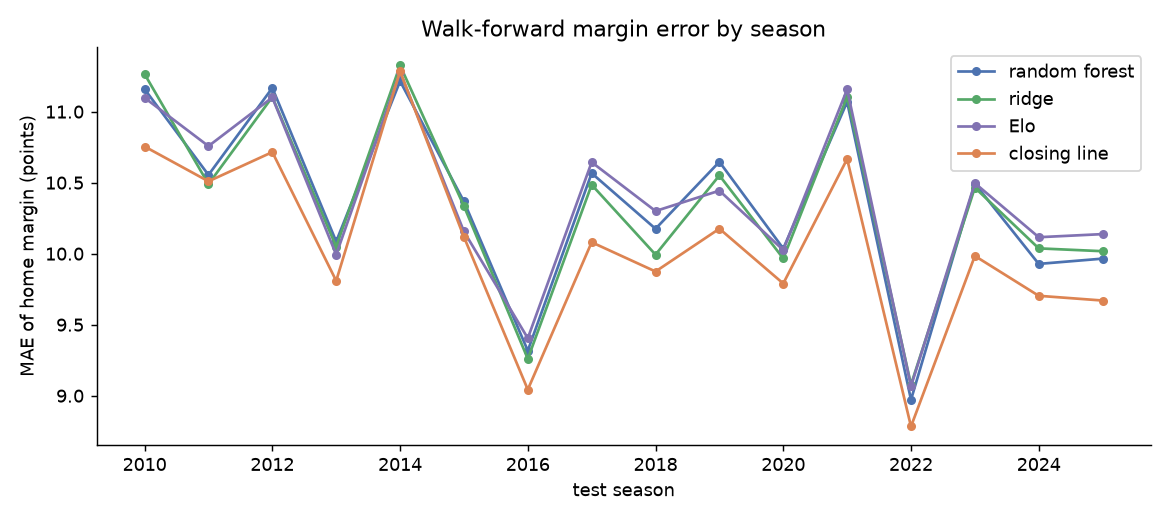
\includegraphics[width=0.95\textwidth]{rf_mae_by_season.png}
\caption{Margin error by test season. All methods share the hard and easy seasons; the closing line is lowest in 15 of 16.}
\label{fig:mae_season}
\end{figure}

\begin{figure}[H]
\centering
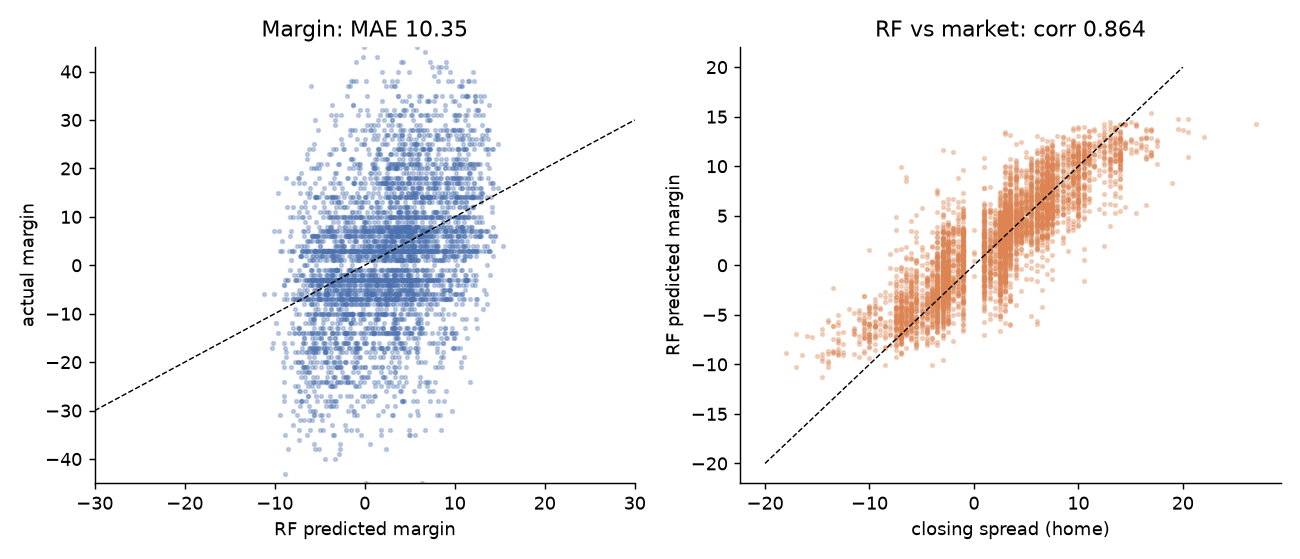
\includegraphics[width=0.95\textwidth]{rf_pred_vs_actual.png}
\caption{Left: predicted against actual margin. Right: the forest's margin against the closing spread (correlation 0.86).}
\label{fig:pred_actual}
\end{figure}

\paragraph{The two-output structure.}

Because the forest predicts a point in the $(h,a)$ plane, its residuals describe a two-dimensional distribution around that point (Table~\ref{tab:bivariate}, Figure~\ref{fig:bivariate}). The correlation between the home and away residuals is 0.01: once the two means are set, the leftover error in one score says nothing about the other. Residual spread grows with the predicted score, so high-scoring games are less predictable in points, as a Poisson-like scoring process implies. Calibration per score is good: when the forest predicts 20 points the team scores 20 on average, across the range 15 to 33.

\begin{table}[H]
\centering
\small
\begin{tabular}{lcc}
\toprule
\textbf{Quantity} & \textbf{Home} & \textbf{Away} \\
\midrule
Standard deviation of the actual score & 10.21 & 9.83 \\
Standard deviation of the residual & 9.64 & 9.36 \\
Range of predicted scores & 15.8 to 33.3 & 13.3 to 30.4 \\
Residual s.d., lowest third of predictions & 9.20 & 8.88 \\
Residual s.d., highest third of predictions & 10.11 & 9.76 \\
\bottomrule
\end{tabular}
\caption{Residual structure of the two-output forest, 4,363 out-of-sample games. Residual correlation 0.011.}
\label{tab:bivariate}
\end{table}

\begin{figure}[H]
\centering
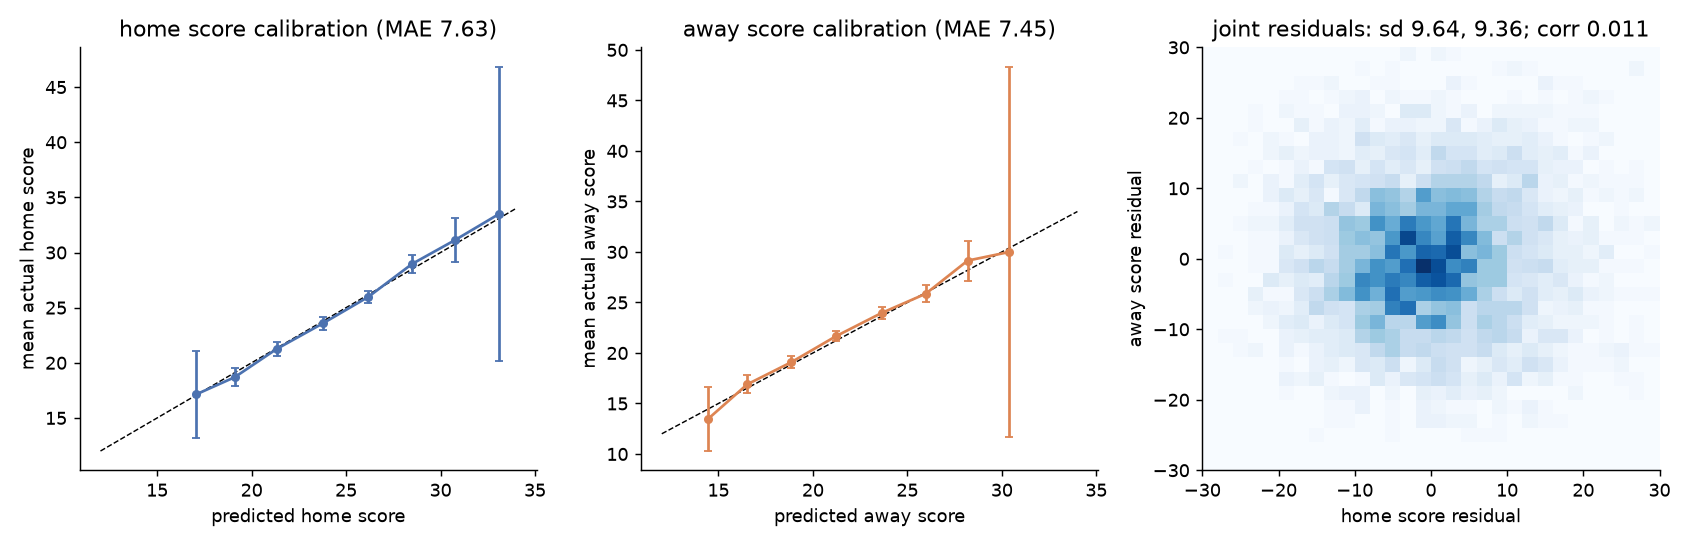
\includegraphics[width=0.98\textwidth]{rf_bivariate.png}
\caption{Calibration of the home and away score predictions and the joint distribution of the two residuals.}
\label{fig:bivariate}
\end{figure}

These residual statistics are the parameters $(\sigma_h,\sigma_a,\rho)$ of the probabilistic extension suggested by Professor Amine. Table~\ref{tab:bivariate} and Figure~\ref{fig:bivariate} pool the residuals of all sixteen test seasons, which is the right thing for describing them but not for scoring probabilities on those same seasons. For scoring we refit them walk-forward: the probability for a game in season $t$ uses the residual standard deviations and correlation of the out-of-sample predictions for seasons $2010$ to $t-1$ only, so the first scored season, 2016, uses six seasons of residuals (1,602 games) and 2025 uses fifteen (4,078). The margin standard deviation estimated this way runs from 13.87 (for 2016) down to 13.40 (for 2025), against 13.36 pooled. Used as a bivariate normal around the two predicted scores, the fold-wise residuals give a home-win probability with Brier score 0.2208 over 2016--2025 (0.2207 with the pooled values), against 0.2220 for Elo and 0.2108 for the de-vigged moneyline. The empirical grid used for the alternative, placing the two predicted means on the score table of Section~\ref{sec:pricing}, was already fold-wise: its prior for season $t$ is the table of all games before $t$, and it gives 0.2213. The probabilities are calibrated (Figure~\ref{fig:rf_cal}); the gap to the market is in sharpness, not bias.

{\color{red}\textbf{Amine comment:} Please confirm that residual covariance and the empirical grid use only earlier games in each test fold. Their stated estimation periods overlap the evaluation years.}

{\color{blue}\textbf{Sai comment:} Fixed. The grid prior was already fold-wise (all games before the test season). The residual covariance was pooled; it is now refit walk-forward from seasons before each test season, as the paragraph above reports (Brier 0.2208 fold-wise against 0.2207 pooled), and the pooled table and figure are labelled as descriptive.}

\begin{figure}[H]
\centering
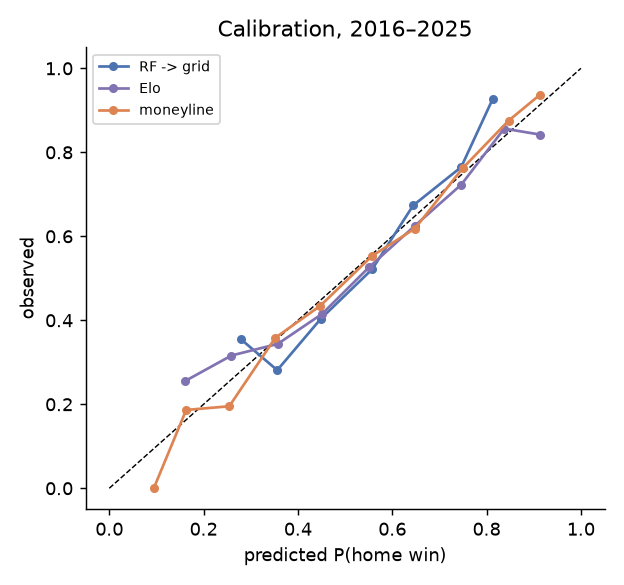
\includegraphics[width=0.5\textwidth]{rf_calibration.png}
\caption{Calibration of home-win probabilities, 2016--2025.}
\label{fig:rf_cal}
\end{figure}

\paragraph{What the forest uses.}

Averaged over the sixteen fits, the five most important features are all team-strength summaries from results: the difference in opponent-adjusted weighted margin, the difference in weighted margin, and the three Elo features (Figure~\ref{fig:importance}). The first play-by-play feature is yards per play, followed by the starting quarterback's success rate and EPA per dropback and points per drive. Injury, rest and weather features are far down the list. Most of what the model knows is how good each team has been; the efficiency and quarterback features refine that at the margin. The forest used all 759 features with no selection or tuning and matched a regularised linear model, which is what Professor Shasha expected.

\begin{figure}[H]
\centering
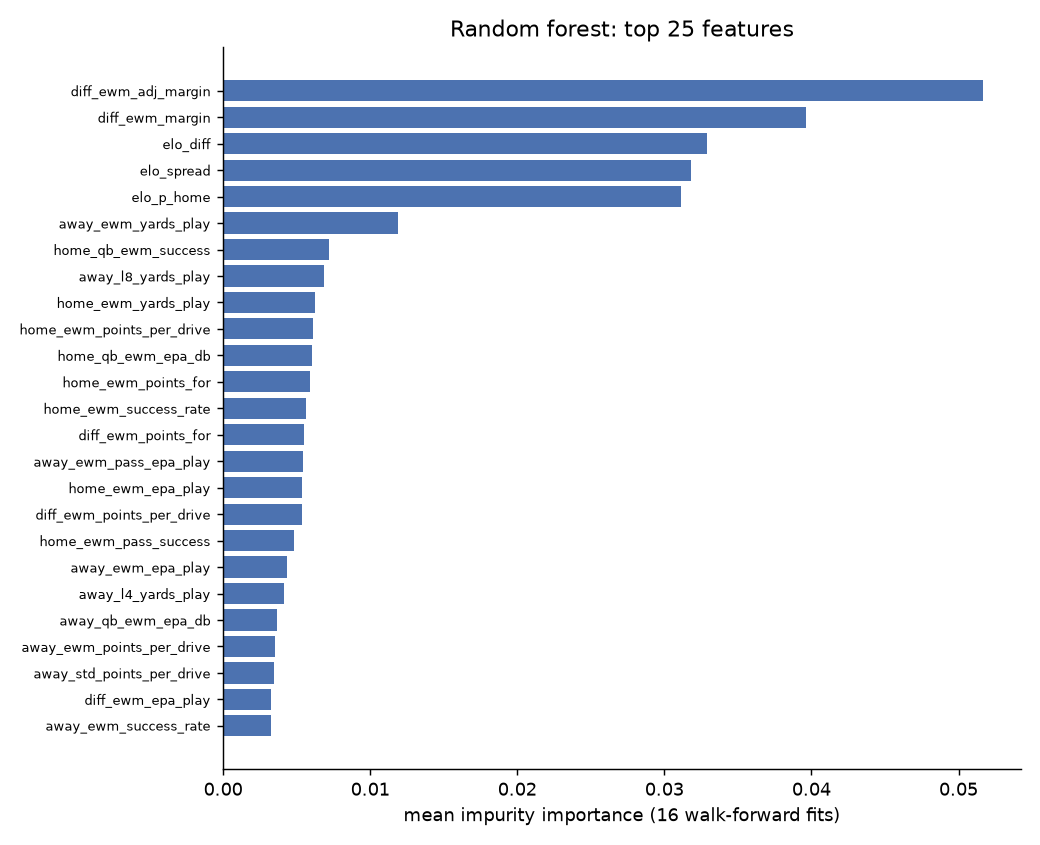
\includegraphics[width=0.75\textwidth]{rf_importance.png}
\caption{Top 25 features by mean impurity importance over the sixteen walk-forward fits.}
\label{fig:importance}
\end{figure}

